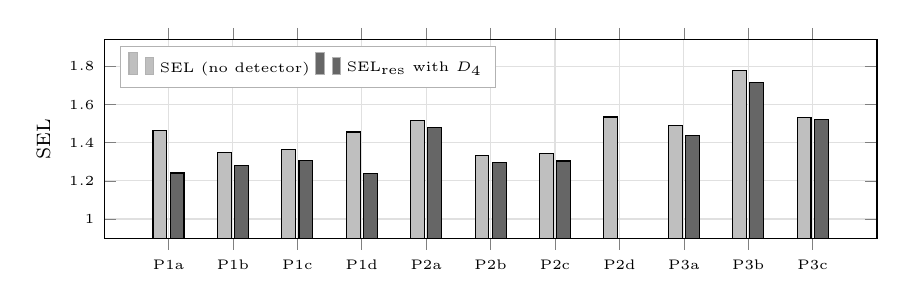
\begin{tikzpicture}
\begin{axis}[
  width=0.94\columnwidth, height=4.1cm,
  ybar=1.2pt, bar width=5pt,
  ylabel={SEL},
  symbolic x coords={P1a,P1b,P1c,P1d,P2a,P2b,P2c,P2d,P3a,P3b,P3c},
  xtick=data, ymin=0.90, ymax=1.94,
  grid=both, grid style={black!12},
  legend style={at={(0.02,0.97)},anchor=north west,font=\tiny,
                draw=black!30,legend columns=2},
  label style={font=\scriptsize}, tick label style={font=\tiny}
]
\addplot[fill=black!25] coordinates {(P1a,1.464) (P1b,1.350) (P1c,1.365) (P1d,1.456) (P2a,1.515) (P2b,1.331) (P2c,1.344) (P2d,1.535) (P3a,1.491) (P3b,1.777) (P3c,1.530)};
\addlegendentry{$\mathrm{SEL}$ (no detector)}
\addplot[fill=black!60] coordinates {(P1a,1.241) (P1b,1.281) (P1c,1.305) (P1d,1.238) (P2a,1.482) (P2b,1.298) (P2c,1.304) (P2d,0.890) (P3a,1.439) (P3b,1.718) (P3c,1.520)};
\addlegendentry{$\mathrm{SEL_{res}}$ with $D_4$}
\end{axis}
\end{tikzpicture}
%(P1a,1.464) +- (0,0.013) (P1b,1.350) +- (0,0.013) (P1c,1.365) +- (0,0.011) (P1d,1.456) +- (0,0.011) (P2a,1.515) +- (0,0.015) (P2b,1.331) +- (0,0.009) (P2c,1.344) +- (0,0.016) (P2d,1.535) +- (0,0.017) (P3a,1.491) +- (0,0.014) (P3b,1.777) +- (0,0.022) (P3c,1.530) +- (0,0.015)
